\subsection{Licht als Welle}
\label{sec:welle}
Licht hat sowohl die Eigenschaften eines klassischen Teilchens, als auch die einer klassischen Welle -- es unterliegt also dem Prinzip des \emph{Welle-Teilchen-Dualismus} der Quantenphysik. Das sich Licht wie eine Welle verhält, zeigt sich im Experiment besonders anschaulich an seinem Verhalten, wenn es auf eine Öffnung (in einem ansonsten lichtundurchlässigen Hindernissen) trifft, deren Durchmesser innerhalb einiger Größenordnungen der Wellenlänge liegt. Dort tritt Beugung auf und es kann ein für Wellenphänomene typisches Beugungsmuster der Intensität gemessen werden. Die Gesetze der geometrischen Optik erklären dieses Verhalten nicht, da sich Lichtstrahlen in diesem Modell nicht gegenseitig beeinflussen können. Damit wird sowohl Interferrenz, als auch Beugung ausgeschlossen. Von Beugung wird daher gesprochen, wenn die Ausbreitung des Lichtes von diesen Gesetzen abweicht. Auch die Betrachtung von Licht als klassische Welle stellt nur eine Näherung dar, da es sich eigentlich nur mit der Quantenmechanik beschreiben lässt. Breitet sich Licht im Vakuum aus, ist es allerdings möglich den Mittelwert über eine große Anzahl von Lichtquanten zu bilden, wodurch die Näherung des Lichts als Welle anwendbar wird.

Betrachtet man Licht also als Welle, kann das \emph{Huygenssche Prinzip} auf ihr Ausbreitungsverhalten angewendet und als Erklärung für das Auftreten von Beugung verwendet werden. Das Prinzip besagt, dass jeder Punkt einer Wellenfront als Ursprung einer neuen kugelförmigen \emph{Elementarwelle} gleicher Phase interpretiert werden kann. Die Einhüllende aller dieser Elementarwellen bestimmt die Wellenfront für jeden späteren Zeitpunkt. Für die Beschreibung eines bestimmten Punktes der Wellenfront zu einem festgelegten Zeitpunkt müssen daher alle in diesem Zeitpunkt ankommenden Elementarwellen überlagert werden. Die weitere Betrachtung wird nun exemplarisch an einem parallelen Spalt als Öffnung durchgeführt, da mit einem geometrisch einfachem Objekt auch die mathematische Beschreibung vereinfacht wird.

\subsection{Fresnelsche und Fraunhofersche Beugung}

Grundsätzlich kommen zwei in Abbildung~\ref{fig:fresnel} skizzierte Versuchsanordnungen für den Einzelspalt in Frage: Die \emph{Fresnelsche Anordnung}, bei der Lichtquelle und Beobachtungsschirm in endlicher Entfernung zum Spalt aufgebaut sind, zeigt, dass die Strahlenbündel divergieren und somit auch Strahlen (im selben Punkt) interferieren können, die vorher unterschiedlich stark gebeugt wurden (siehe Skizze~\ref{fig:fresnel}~a).

Auf der anderen Seite gibt es die \emph{Fraunhofersche Anordnung}: Hier liegen Lichtquelle und Beobachtungsschirm quasi im Unendlichen, mit der Folge, dass die Strahlen parallel auf den Spalt treffen und somit eine ebene Wellenfront bilden. Als Konsequenz können nur Strahlen im selben Punkt interferieren, die vorher auch unter dem selben Winkel gebeugt wurden (siehe Skizze~\ref{fig:fresnel}~b). Die mathematische Beschreibung der Fraunhoferschen Beugung ist daher einfacher als die der Fresnelschen Beugung. Im Folgenden wird aus diesem Grund nur noch die Fraunhofersche Anordnung betrachtet.

\begin{figure}
  \centering
  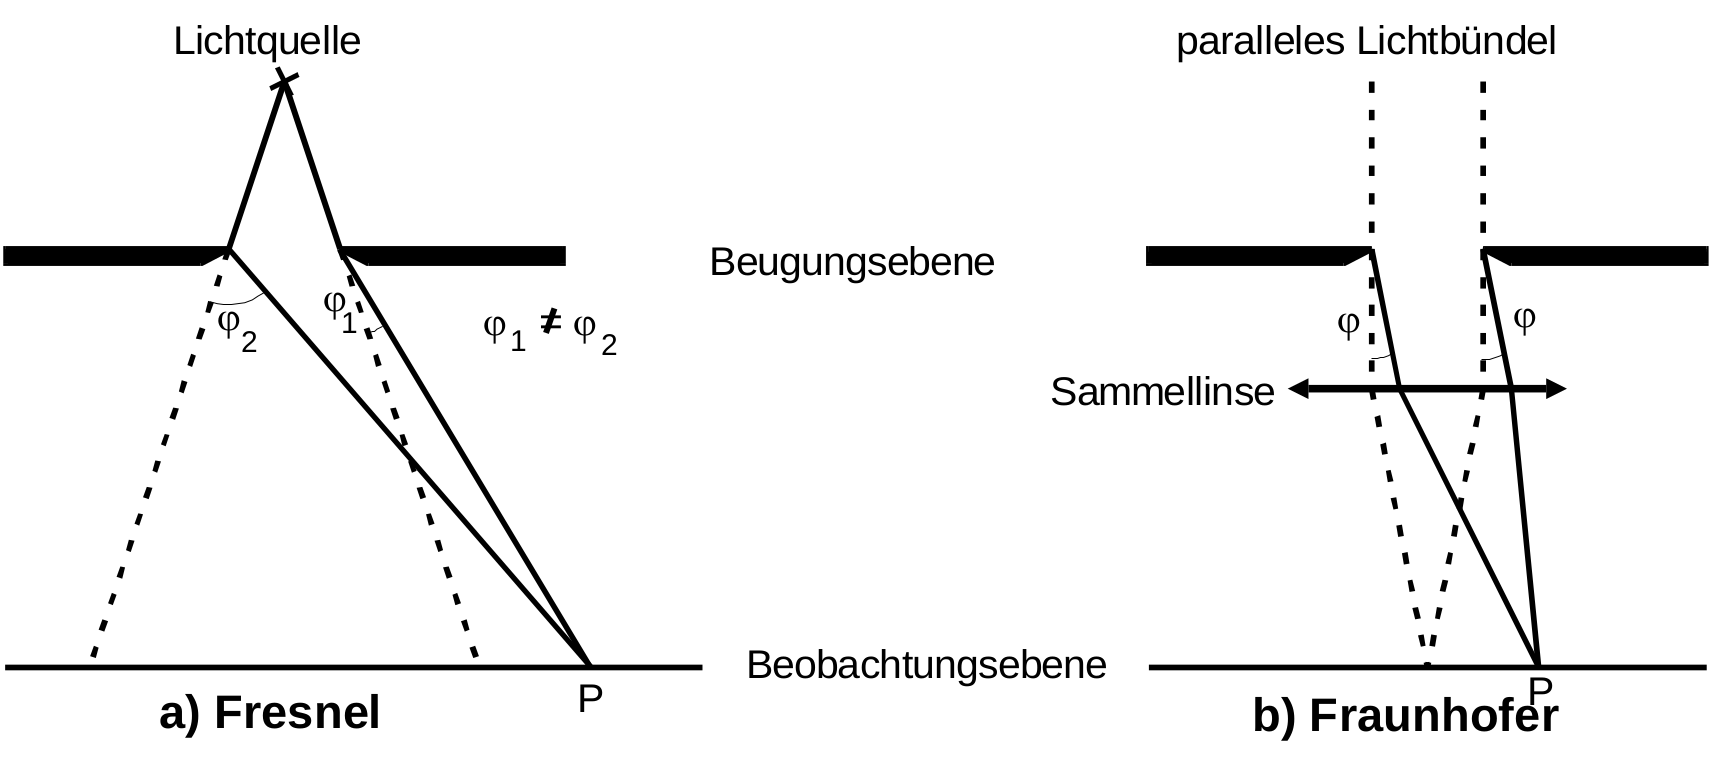
\includegraphics[width=0.6\textheight]{../figures/Fresnel.png}
  \caption{Skizze von Fresnelscher (a) und Fraunhoferscher (b) Beugung am Einzelspalt.[Skript V406]}
\label{fig:fresnel}
\end{figure}

\subsection{Beugung am Einzelspalt}
\label{sec:einzel}
Es wird ein Spalt betrachtet, dessen Breite $b$ sehr viel kleiner ist als seine Länge. Das parallel auftreffende Lichtbündel wird dadurch nur in der x-Richtung durch die Breite des Spalts begrenzt. Der Aufbau ist in Abbildung~\ref{fig:spalt} skizziert.

\begin{figure}
  \centering
  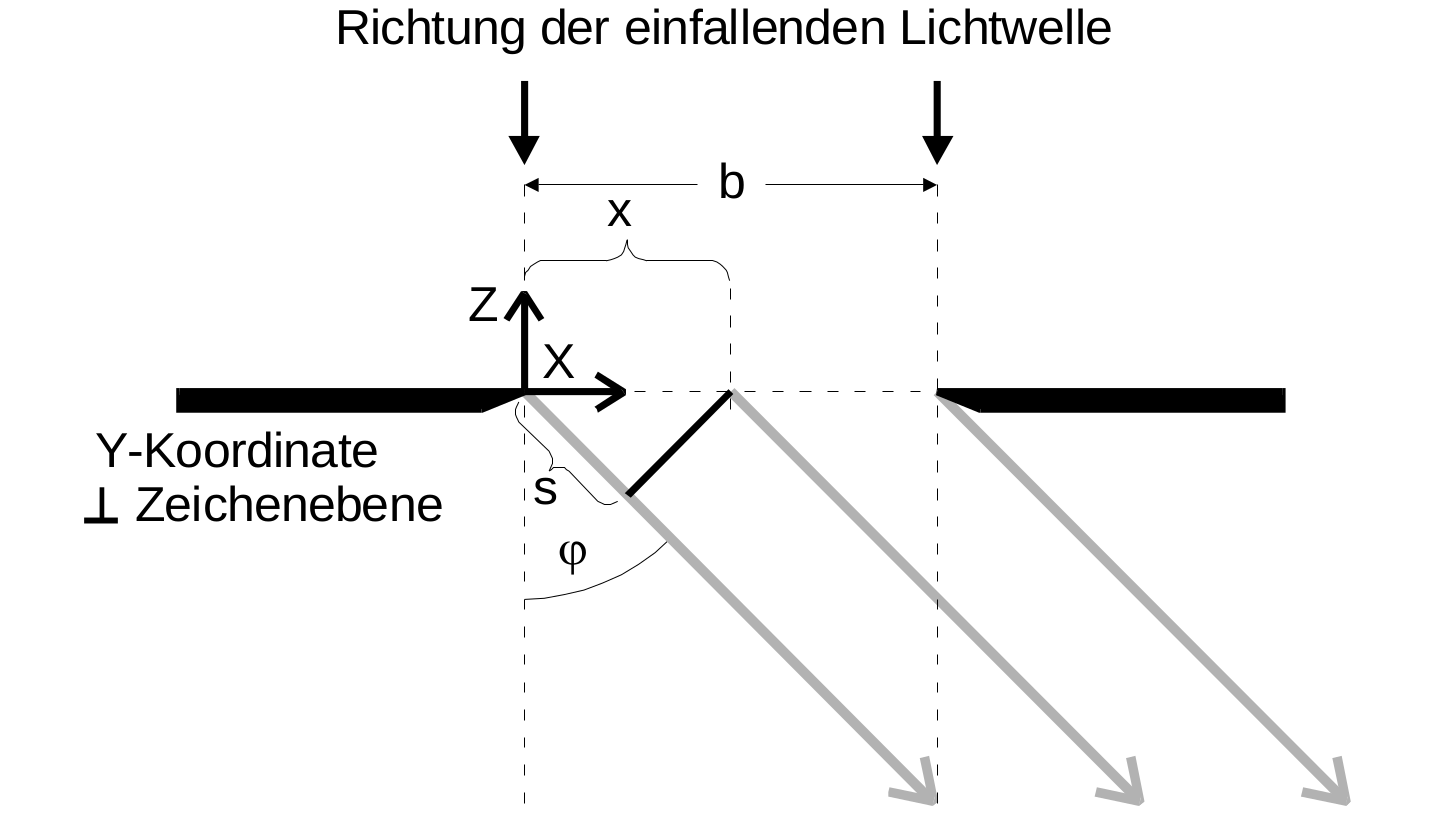
\includegraphics[width=0.4\textheight]{../figures/spalt.png}
  \caption{Skizze eines Einzelspaltes bei Fraunhoferscher Beugung.[Skript V406]}
\label{fig:spalt}
\end{figure}

Auf diesen Spalt trifft eine ebene Welle, die durch die Gleichung
\begin{align}
  A(z,t) = A_0 \exp{(i(\omega t - \frac{2 \pi z}{\lambda}))}
  \label{equ:ebeneWelle}
\end{align}
beschrieben wird. Auf Grund des \emph{Huygensschen Prinzips} ist klar, dass die Welle an diesem Spalt gebeugt wird. Um die Feldstärke an einem Punkt bestimmen zu können, muss nach Abschnitt~\ref{sec:welle} über alle Strahlenbündel summiert werden, die unter dem selben Winkel~$\varphi$ abgelenkt werden. Der Abstand dieser Strahlenbündel betrage $x$. Abbildung~\ref{fig:spalt} verdeutlicht, dass der Phasenunterschied zwischen den Strahlenbündeln
\begin{align}
  \delta = \frac{2 \pi s}{\lambda} = \frac{2 \pi x \sin{\varphi}}{\lambda}
  \label{equ:delta}
\end{align}
beträgt. Der Abstand der Strahlenbündel ist allerdings infinitesimal klein, daher muss die Summe in eine Integration über die gesamte Spaltbreite $b$ übergehen. Die Feldstärke der in $\varphi$-Richtung abgelenkten Strahlenbündel kann also durch
\begin{align}
  B(z,t,\varphi) = A_0 \int_0^b \exp{(i(\omega t - \frac{2 \pi z}{\lambda} + \delta))} \mathrm dx
\end{align}
beschrieben werden.
Die Integration sowie einige Umformungsschritte führen für die Feldstärke $B$ auf
\begin{align}
  B(z,t,\varphi) = A_0 \exp{(i(\omega t - \frac{2 \pi z}{\lambda}))} \exp{( \frac{i \pi b \sin{\varphi}}{\lambda})} \frac{\lambda}{\pi \sin{\varphi}} \sin{(\frac{\pi b \sin{\varphi}}{\lambda})} \; .
  \label{equ:B}
\end{align}
Die Orts- und Zeitabhängigkeit der Feldstärke in Ausbreitungsrichtung wird in Gleichung~\eqref{equ:B} durch die erste Exponentialfunktion beschrieben. Die zweite Exponentialfunktion ist ein Phasenfaktor, der von der Richtung abhängig ist. Es handelt sich also lediglich um zwei Phasenfunktionen, die für die Intensitätsmessung keine Bedeutung haben. Die Feldstärke $B$ lässt sich aufgrund der hohen Frequenz des Lichts nicht unmittelbar messen, für eine experimentelle Untersuchung ist daher nur die zeitlich gemittelte Intensität $I(\varphi)$ von Interesse. Sie ist proportional zum Betragsquadrat der Feldstärke
\begin{align}
  I(\varphi) \propto  |B(\varphi)|^2 \; .
\end{align}
Für die Intensität von Licht, das an einem parallelen Einzelspalt gebeugt wurde, folgt daher
\begin{align}
  I(\varphi) = A_0^2 b^2 (\frac{\lambda}{\pi b \sin{\varphi}})^2 \sin^2{(\frac{\pi b \sin{\varphi}}{\lambda})} \; .
  \label{equ:I}
\end{align}
Dabei handelt es sich um einen \emph{Sinus Kardinalis}
\begin{align}
  I(\varphi) \propto \frac{\sin{\chi(\varphi)}}{\chi(\varphi)} \; ,
\end{align}
der die für Beugung typische Intensitätsverteilung liefert (siehe Abbildung~\ref{fig:slit}). Dabei ist $\chi(\varphi) \propto \varphi$.


\subsection{Beugung am Doppelspalt}
Analog zu der Vorgehensweise in Abschnitt~\ref{sec:einzel} kann die Intensitätsverteilung für einen parallelen Doppelspalt berechnet werden. Dafür wird der Doppelspalt als Überlagerung zweier Einzelspalte der Breite $b$ betrachtet, die sich im Abstand $s$ zueinander befinden. Der Aufbau ist in Abbildung~\ref{fig:doppel} skizziert.

\begin{figure}
  \centering
  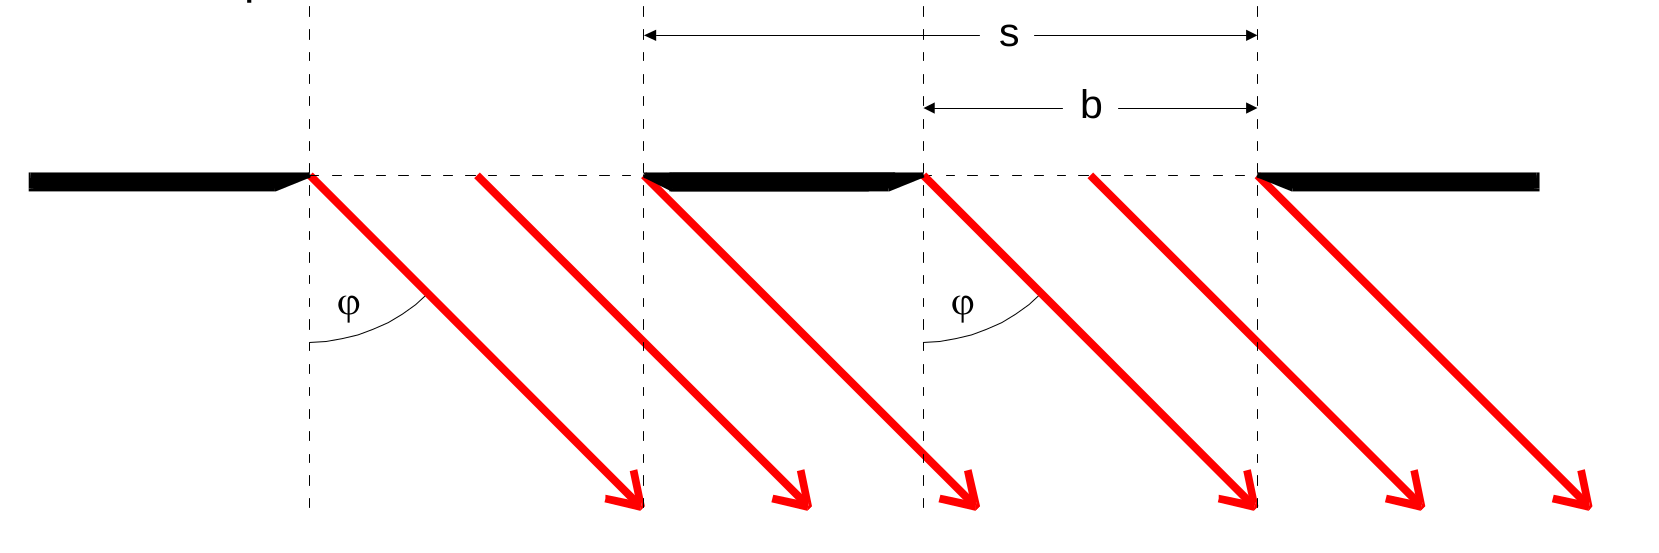
\includegraphics[width=0.4\textheight]{../figures/doppel.png}
  \caption{Skizze eines Doppelspalts bei Fraunhoferscher Beugung.[Skript V406]}
\label{fig:doppel}
\end{figure}

Die Intensitätsverteilung $I(\varphi)$ ergibt sich damit zu
\begin{align}
  I(\varphi) \propto |B(\varphi)|^2 = 4 \cos^2{\frac{\pi s \sin{\varphi}}{\lambda}}(\frac{\lambda}{\pi b \sin{\varphi}})^2 \sin^2{(\frac{\pi b \sin{\varphi}}{\lambda})} \; .
  \label{equ:I_doppel}
\end{align}
Sie unterscheidet sich von der Intensitätsverteilung des Einzelspaltes nur in dem $\cos^2$-Term. Es entsteht also ein ähnliches Bild für die beiden Intensitätsverteilungen. Durch den $\cos^2$-Term ergeben sich aber mehr Minima und Maxima als beim Einzelspalt, dessen Intensitätsverteilung als die Einhüllende der Doppelspaltintensitätsverteilung dargestellt werden kann (siehe Abbildung~\ref{fig:slit}).

\begin{figure}
  \centering
  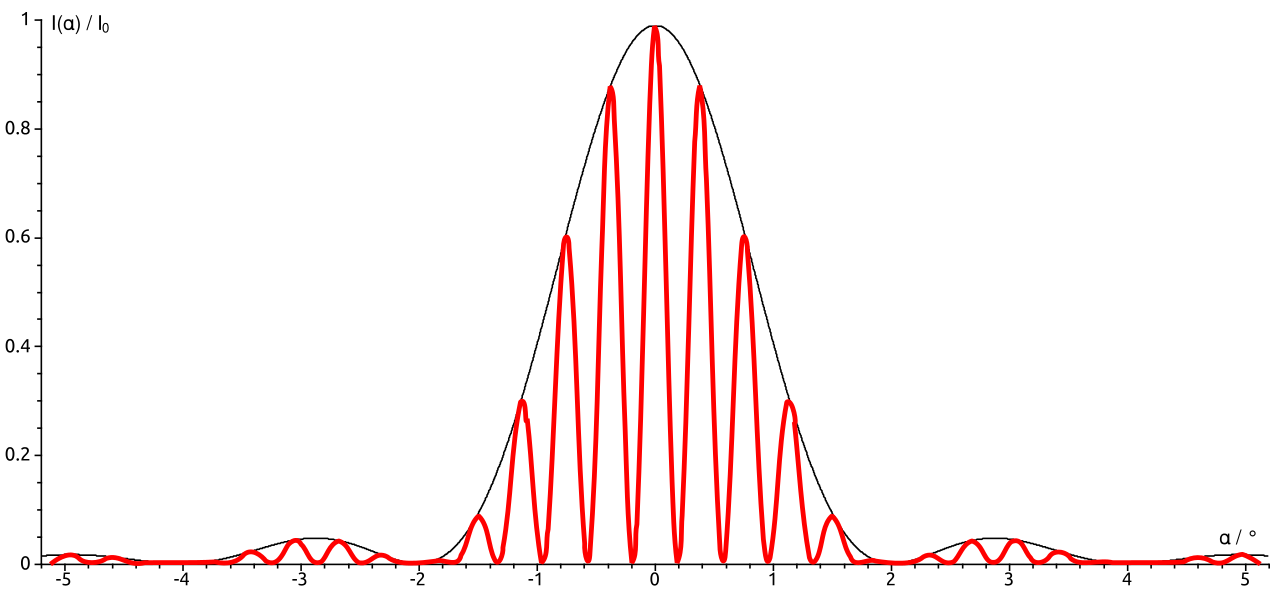
\includegraphics[width=0.4\textheight]{../figures/Slit_double.png}
  \caption{Intensitätsverteilung bei Beugung am Einzelspalt (schwarz) und Doppelspalt (rot). [By Klaus-Dieter Keller]}
\label{fig:slit}
\end{figure}


%This is the end
